%%%%%%%%%%%%%%%%%%%%%%%%%%%%%%%%%%%%%%%%%%%%%%%%%%%%%%%%%%%%%%%%%%%%%%
%     File: ExtendedAbstract_imple.tex                               %
%     Tex Master: ExtendedAbstract.tex                               %
%                                                                    %
%     Author: Andre Calado Marta                                     %
%     Last modified : 27 Dez 2011                                    %
%%%%%%%%%%%%%%%%%%%%%%%%%%%%%%%%%%%%%%%%%%%%%%%%%%%%%%%%%%%%%%%%%%%%%%
% A Calculation section represents a practical development
% from a theoretical basis.
%%%%%%%%%%%%%%%%%%%%%%%%%%%%%%%%%%%%%%%%%%%%%%%%%%%%%%%%%%%%%%%%%%%%%%

\section{Methodology}
\label{sec:imple}
This section outlines the methodology to be applied throughout this study, namely Data Envelopment Analysis (DEA), Truncated Regression, and the Malmquist Productivity Index (MPI). 
\subsection{Data Envelopment Analysis (DEA)}
\label{dea}
DEA is a non-parametric method used to evaluate the efficiency of Decision Making Units (DMUs) that convert inputs into outputs, by comparing each DMU to a best-practice frontier. The calculated efficiency is relative and is
measured by the distance to the frontier, meaning a DMU is efficient if it lies on the frontier, and inefficient if it lies below it. 

DEA models can be oriented in two ways: input or output oriented. In an input-oriented model the focus is on how much the inputs of a DMU can be proportionally reduced, without affecting the outputs
produced. On the other hand, an output-oriented model focuses on increasing output quantities propor-
tionally, while maintaining the same level of inputs \cite{charnes1994}. 

Another important aspect of DEA is the assumption on returns to scale. In this regard there are two
main formulations, the CCR model (Charnes, Cooper, Rhodes) and the BCC model (Banker, Charnes,
Cooper). The first assumes constant returns to scale (CRS), meaning that an increase in inputs will lead to a proportional increase in outputs. The second assumes variable returns to scale (VRS), meaning it separates the inefficiencies due to scale from those due to pure technical inefficiency, and therefore compares DMUs of similar size \cite{banker1984}. 

Even though the CCR model is a valuable measure of overall efficiency, as airports cannot easily adjust their scale, the BCC model is often more appropriate in this context and will, therefore, be the model applied in this work. \eqnref{input_dea} and \eqnref{output_dea} present the formulations for the input-oriented and output-oriented BCC models, respectively. \eqnref{eq:bcc_constraints} and \eqnref{eq:bcc_constraints_output} represent the respective constraints for each model. The main difference between the CCR and BCC models is the inclusion of the convexity constraint (i.e., \(\sum_j \lambda_j = 1\)), which ensures that an inefficient DMU is only benchmarked against similar sized DMUs. 
\begin{center}
\textbf{Input-oriented BCC Model}
\end{center}
\begin{equation}
    \label{input_dea}
min_{\theta,\lambda} \quad \theta
\end{equation}
subject to
\begin{equation}
\label{eq:bcc_constraints}
\begin{gathered}
\sum_j x_{i,j}\lambda_j \leq \theta x_{i,o} \quad \text{for } i=1,\ldots,m \\
\sum_j y_{r,j} \lambda_j \geq y_{r,o} \quad \text{for } r=1,\ldots,s \\
\sum_j \lambda_j = 1 \\
\lambda_j \geq 0
\end{gathered}
\end{equation}

\vspace{0.5cm}
\begin{center}
\textbf{Output-oriented BCC Model}
\end{center}
\begin{equation}
    \label{output_dea}
max_{\phi,\lambda} \quad \phi
\end{equation}
subject to
\begin{equation}
\label{eq:bcc_constraints_output}
\begin{gathered}
\sum_j y_{r,j} \lambda_j \geq \phi y_{r,o} \quad \text{for } r=1,\ldots,s \\
\sum_j x_{i,j}\lambda_j \leq x_{i,o} \quad \text{for } i=1,\ldots,m \\
\sum_j \lambda_j = 1 \\
\lambda_j \geq 0
\end{gathered}
\end{equation}

Having obtained the efficiency scores using both the CCR and BCC models,
it is possible to obtain the scale efficiency (SE) of an airport. SE measures the loss that a DMU suffers
for not operating at optimal scale, and it is calculated as the ratio between the efficiency scores obtained
using CRS and VRS \cite{bogetoft2011}:

\begin{equation}
    \label{eq:scale_efficiency}
SE = \frac{E_{CRS}}{ E_{VRS}}
\end{equation} 

The value of SE, is always between 0 and 1, since the efficiency score obtained using the CCR model is always less than or equal to that obtained using the BCC model. An SE value of 1 indicates that the DMU is operating at optimal scale, while a value less than 1 indicates that it is not.

Analyzing the value of SE does not provide information on the type of scale inefficiency, i.e., whether
the DMU is operating at increasing or decreasing returns to scale. To identify the nature of the returns to
scale, another model as to be used: the non-increasing returns to scale (NIRS) model, which is derived
from the BCC model by replacing the \(\sum_j \lambda_j = 1\) restriction with \(\sum_j \lambda_j \leq 1\) \cite{coelli2005}. \eqnref{eq:rts_definition} summarizes the classification criteria for the different RTS that can be identified
by comparing the models explained above \cite{huguenin2012}.

\begin{equation}
\label{eq:rts_definition}
RTS =
\begin{cases}
IRS, & \text{if } E_{NIRS} \neq E_{VRS} \\
CRS, & \text{if } E_{NIRS} = E_{VRS} = E_{CRS} \\
DRS, & \text{if } E_{NIRS} = E_{VRS} \neq E_{CRS}
\end{cases}
\end{equation}
 
Efficiency scores obtained using DEA can be influenced not only by management decisions and scale
operation conditions, but also by different exogenous factors. Second-stage regressions are usually
applied to identify the effect of these factors, in which the DEA efficiency values obtained in the first
stage are regressed against a set of potential explanatory variables. In this study, a truncated regression
is going to be applied.

\subsection{Truncated Regression} 
\label{truncreg}

Following \cite{simar2007}, a double bootstrapping procedure is applied in the second-stage
truncated regression that is given by:
\begin{equation}
\label{eq:regression}
\hat{\theta_i}=\alpha+\beta Z_i + \varepsilon_i, \quad i=1,\ldots,n   
\end{equation}
where
\begin{equation}
\label{eq:noise}
\varepsilon_i \sim N(0, \sigma_\varepsilon^2), \quad \text{such that} \quad \varepsilon_i \geq 1 - \alpha - Z_i \beta
\end{equation}
which is estimated by maximizing the corresponding likelihood function.

$\hat{\theta_i}$ represents the bias corrected efficiency value of the $n$ DMUs, $\alpha$ a constant term, $\beta$ the vector of
regression coefficients, $Z_i$ a set of explanatory variables used to evaluate the efficiency scores and $\varepsilon_i$ a
random variable accounting for statistical noise. 

In previous efficiency studies employing DEA, a common practice for estimating the model in \eqnref{eq:regression} had been to employ a censored regression (Tobit). However, \cite{simar2007} demonstrated that this approach is inappropriate because efficiency scores are always higher than 0 and below or equal to 1, meaning the data is truncated at this value rather than censored. Consequently, using a censored regression model would lead to a bias in the estimation.

Since the DEA efficiency scores are relative and not absolute, there is a strong statistical depen-
dency between each observation. Therefore, using them directly in a second-stage regression may
violate fundamental assumptions of regression analysis, such as the independence of the dependent
variable. To overcome the above problems, the bootstrap technique is applied. The double bootstrap approach proposed
by \cite{simar2007} enables consistent inference in the second stage regression, by addressing
the dependency problem, while simultaneously correcting for bias and estimating variance and confidence intervals. 
To facilitate the interpretation of the required steps and their sequential order for the implementation
of algorithm 2 of \cite{simar2007}, \autoref{fig:simarwilson} provides a flowchart detailing the 7-step procedure.

\begin{figure}[H]
\centering
\begin{tikzpicture}[
  node distance=4mm,
  box/.style={
    rectangle, draw, rounded corners,
    text width=60mm, inner sep=2mm, font=\small,
    align=center
  },
  arrow/.style={->, thick}
]
  % Flowchart nodes
  \node[box] (s1) {\textbf{Step 1}\\ Estimate the biased efficiency scores $\theta_i$};
  \node[box, below=of s1] (s2) {\textbf{Step 2}\\ Regress $\theta_i$ to obtain the biased\\ estimations of $\beta$ and $\sigma_\varepsilon$};
  \node[box, below=of s2] (s3) {\textbf{Step 3}\\ Bootstrap $L_1=500$ times to obtain the \\bootstrapped efficiency estimates \\$\theta_i^*$, $\mathcal{B}_i=\{\theta_{i,b}^*\}_{b=1}^{L_1}$};
  \node[box, below=of s3] (s4) {\textbf{Step 4}\\ Calculate the bias using $\mathcal{B}_i$ and $\theta_i$ \\ and compute bias corrected efficiency \\ scores $\hat{\theta}_i$ using $\hat{\theta}_i=\theta_i-\mathrm{BIAS}$};
  \node[box, below=of s4] (s5) {\textbf{Step 5}\\ Re-estimate the truncated regression \\ using the bias corrected efficiency\\ scores $\hat{\theta}_i$, obtaining $\hat{\beta}$ and $\hat{\sigma}_\varepsilon$};
  \node[box, below=of s5] (s6) {\textbf{Step 6}\\ Bootstrap $L_2=2000$ times to obtain\\ a bootstrapped set of $\hat{\beta}^*$ and $\hat{\sigma}_\varepsilon^*$\\ estimates, $\mathcal{C}=\{(\hat{\beta},\hat{\sigma}_\varepsilon)_b\}_{b=1}^{L_2}$};
  \node[box, below=of s6] (s7) {\textbf{Step 7}\\ Using $\mathcal{C}$ and the original estimates $\hat{\beta}$ \\ and $\hat{\sigma}_\varepsilon$, construct the confidence intervals};

  % Flow arrows
  \draw[arrow] (s1) -- (s2);
  \draw[arrow] (s2) -- (s3);
  \draw[arrow] (s3) -- (s4);
  \draw[arrow] (s4) -- (s5);
  \draw[arrow] (s5) -- (s6);
  \draw[arrow] (s6) -- (s7);
\end{tikzpicture}
\caption{Algorithm 2 flowchart based on \cite{simar2007}.}
\label{fig:simarwilson}
\end{figure}

\subsection{Malmquist Productivity Index (MPI)}
\label{mpi}

 Although the DEA methodology provides an accurate
static measure of relative efficiency for each year, it does not fully capture how productivity evolves over
time. To address this limitation, the Malmquist Productivity Index (MPI) is also applied, to provide a
dynamic perspective on efficiency changes.

MPI evaluates the productivity change of a DMU, in our case an airport, by calculating the ratio of
the distance to the frontier in two different time periods, t and t + 1, relative to a common reference
technology. Initially, \cite{caves1982} defined the MPI as follows:

\begin{equation}   
    \label{eq:MI1} 
M_{CCD,\,t} = \frac{D^{t}_{o}\left(x_{t+1}, y_{t+1}\right)}{D^{t}_{o}\left(x_{t}, y_{t}\right)}         
\end{equation}




where $\left(x^{t+1}, y^{t+1}\right)$ represents the input/output combination for the $t+1$ period, and $\left(x^{t}, y^{t}\right)$  for the $t$ period. $D^{t}_{o}\left(x^{t+1}, y^{t+1}\right)$ and $D^{t}_{o}\left(x^{t}, y^{t}\right)$ would then be the distance between the DMU observation in $t+1$ and $t$ periods, respectively, and the best practice frontier in the $t$ period, for airport $o$. 

If one wants to consider the technology from the t + 1 period as the reference, the distance would be measured to the frontier in t + 1 period, meaning $D^{t}_{o}$ would be replaced by $D^{t+1}_{o}$, in the functions of \eqnref{eq:MI1}. To provide a visual illustration of the distance functions defined above, \autoref{fig:fronteiras_malmquist} displays the MPI
distance functions, for $\text{DMU}_\text{X}$, when considering an input orientation.

\begin{figure}[H]
  \centering
  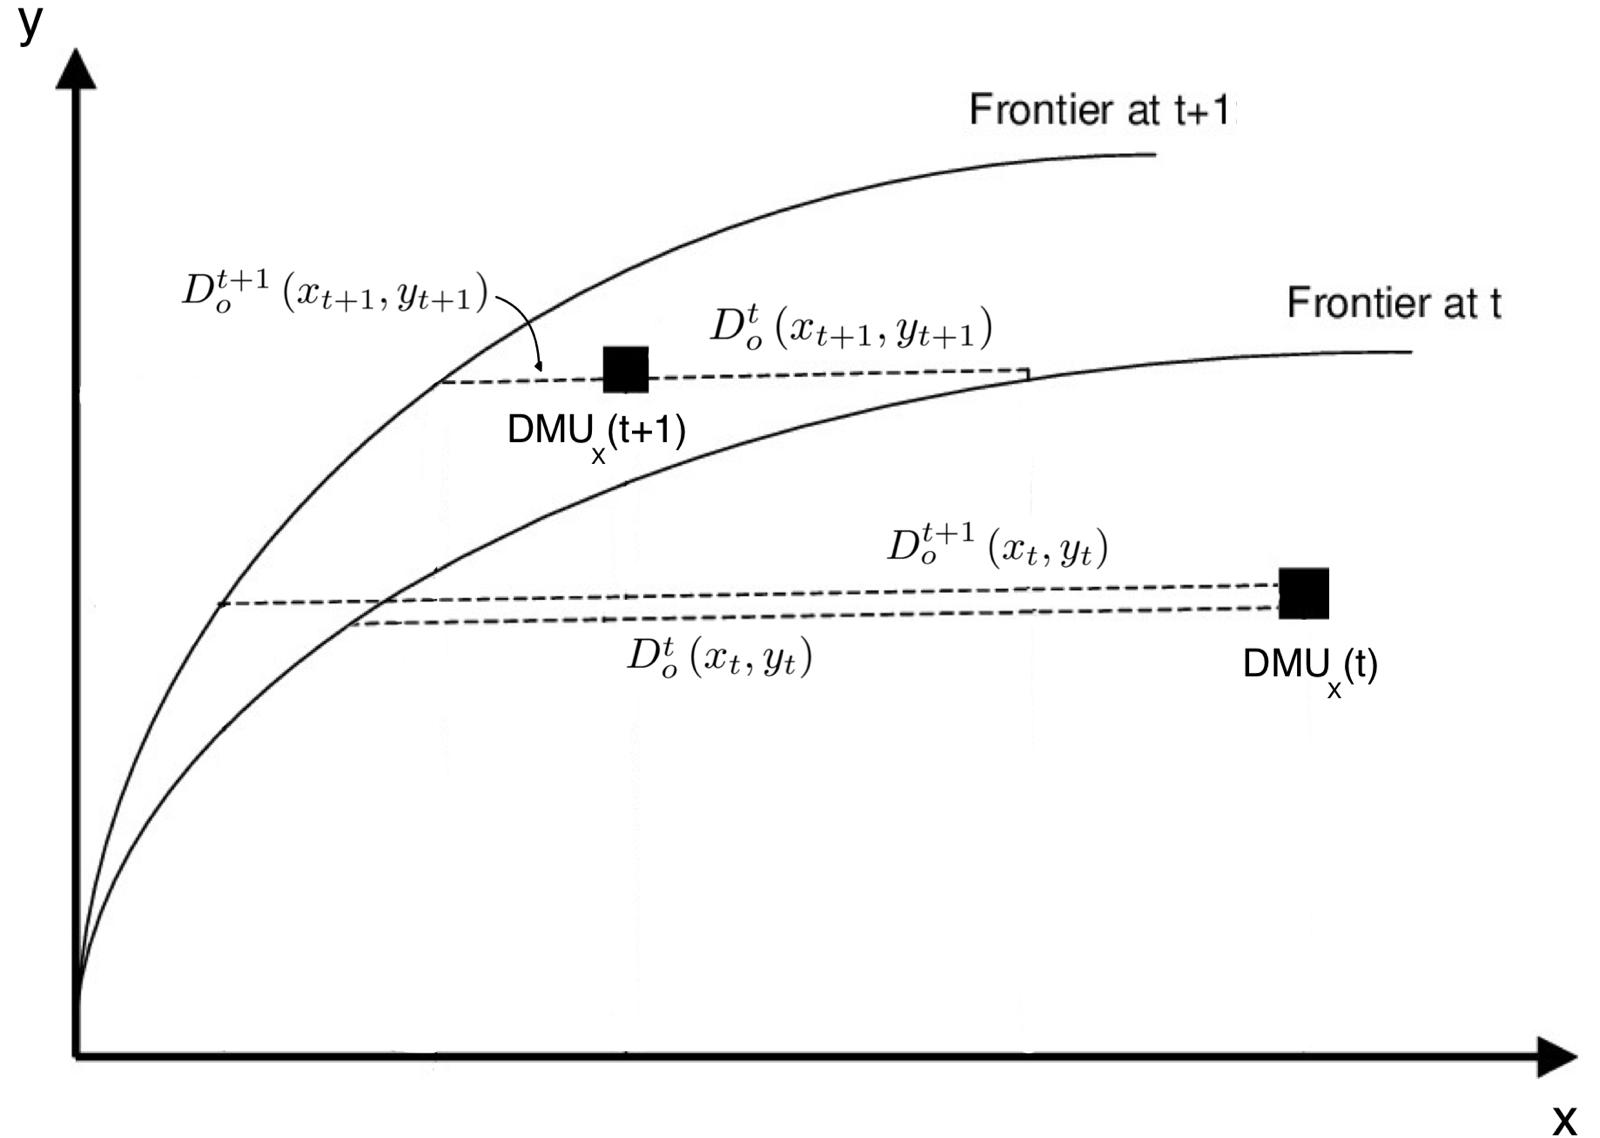
\includegraphics[width=7.5cm]{images/fronteiras_malmquist.jpg}
  \vspace{-0.5cm}
  \caption{Malmquist Productivity Index distance functions for $\text{DMU}_\text{X}$.}
  \label{fig:fronteiras_malmquist}
\end{figure}

In order to avoid the arbitrary selection of a reference technology, \cite{fare1994} specified the
output-based MPI as the geometric mean of the index from \eqnref{eq:MI1}, using both reference technologies, given by:

\begin{equation}
    \label{eq:MI3}
\resizebox{1\linewidth}{!}{$MPI_{o} = \left[ \left( \frac{D^{t}_{o}(x_{t+1}, y_{t+1})}{D^{t}_{o}(x_{t}, y_{t})} \right) \left( \frac{D^{t+1}_{o}(x_{t+1}, y_{t+1})}{D^{t+1}_{o}(x_{t}, y_{t})} \right) \right]^{1/2}$}
\end{equation}

According to \cite{fare1994},  an equivalent way of writing the index of \eqnref{eq:MI3} is:


\begin{equation}
\label{eq:MPI}
\begin{aligned}
MPI_{o} &= \underbrace{\frac{D^{t+1}_{o}(x_{t+1}, y_{t+1})}{D^{t}_{o}(x_{t}, y_{t})}}_{\text{Efficiency Change (EC)}} \\
&\times \underbrace{\left[ 
\frac{D^{t}_{o}(x_{t+1}, y_{t+1})}{D^{t+1}_{o}(x_{t+1}, y_{t+1})} 
\times 
\frac{D^{t}_{o}(x_{t}, y_{t})}{D^{t+1}_{o}(x_{t}, y_{t})} 
\right]^{1/2}}_{\text{Technological Change (TC)}}
\end{aligned}
\end{equation}


This formulation decomposes \eqnref{eq:MI3} into two different components: Efficiency change (EC)
and Technological change (TC). The former evaluates if the airport’s efficiency is getting closer or further
away from the best practice frontier (catching-up effect). The latter captures shifts in the frontier itself,
indicating whether there has been technological progress or regress over time.

So far, the analysis has been conducted under constant returns to scale (CRS). However, the first
term (EC) can be further decomposed into Pure Efficiency Change (PEC), associated with VRS, and
Scale Efficiency Change (SEC). To obtain this full decomposition, two additional programming problems are required, namely the
calculation of Dt+1
o
(xt+1, yt+1) and Dt
o(xt, yt) under VRS, which provides the value of PEC and allows
the calculation of SEC, following the definition of \eqnref{eq:scale_efficiency}. 

A $MPI_{o}$ greater than one indicates an improvement in efficiency between periods t and t + 1. The
same interpretation applies to the other all the other components of the MPI. Conversely, a value less
than one indicates a decline in efficiency